\subsection{Begriffserklärung}
\label{subsec_MLBegriff}
\begin{wrapfigure}{r}{0.5\textwidth}
    \centering
    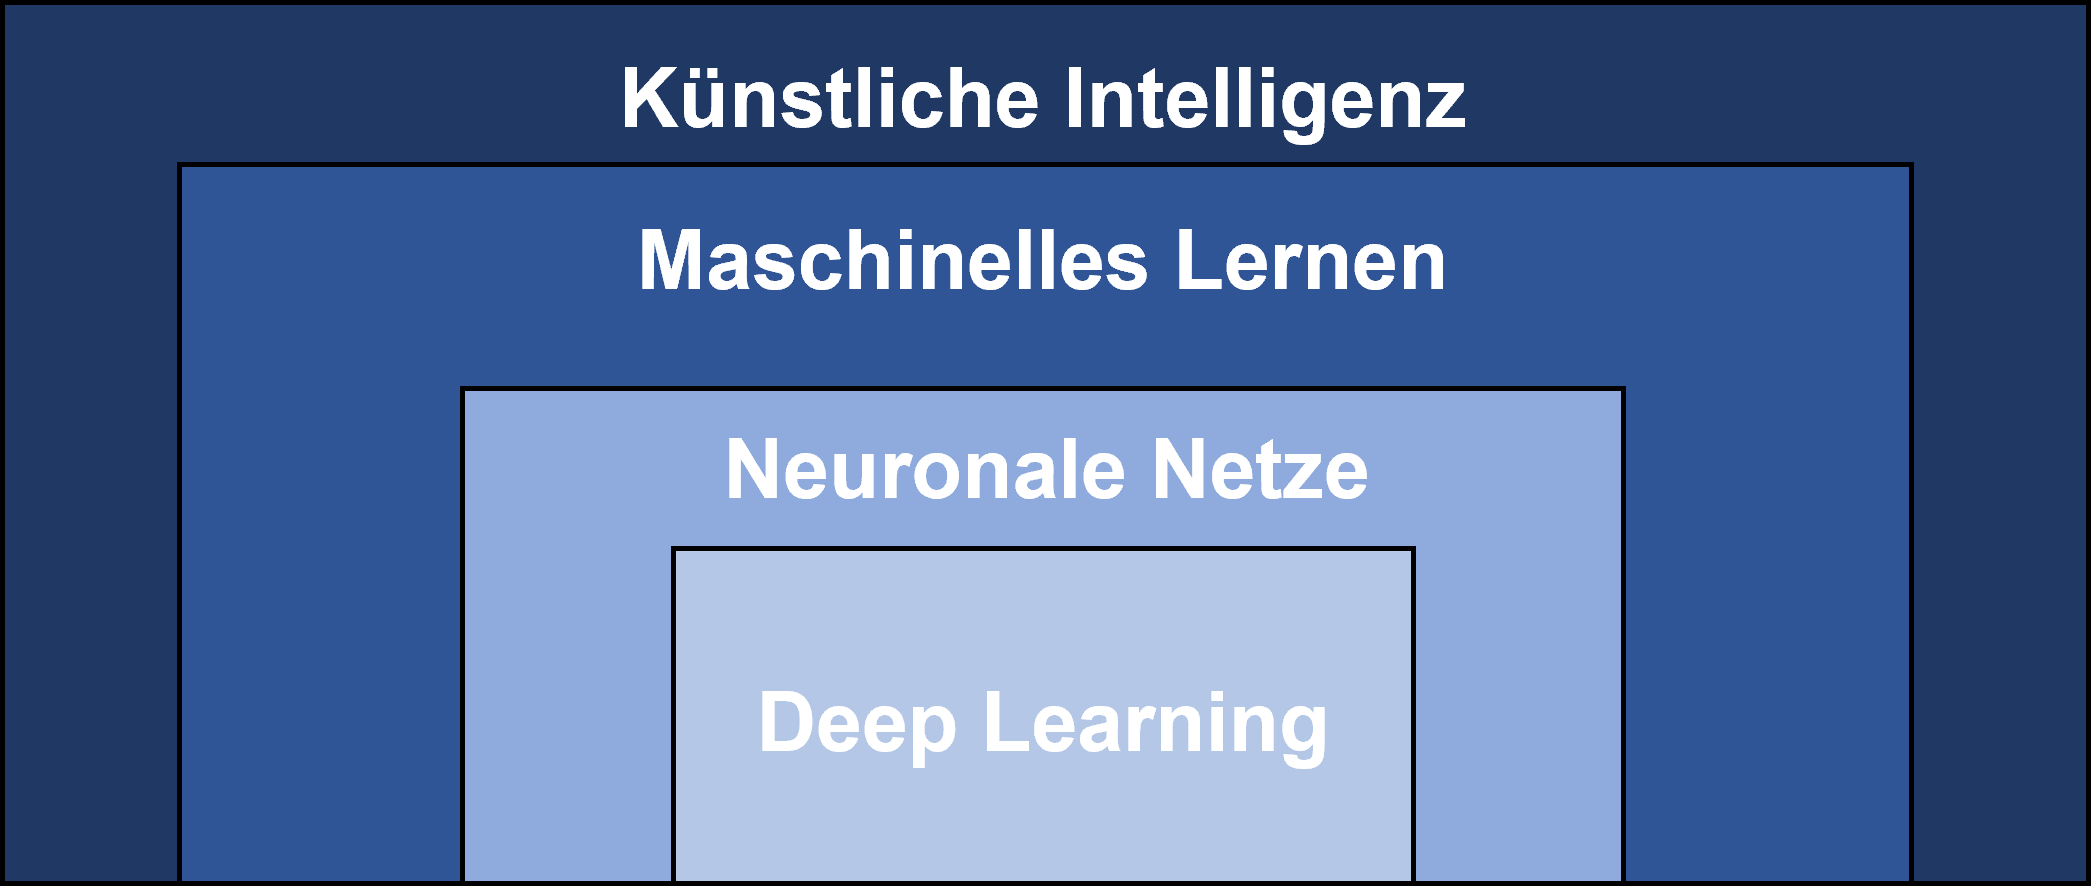
\includegraphics[scale=0.52]{pic/MA-Bilder/KI-ML-DL.PNG}
    \caption{Feld des MLs, eigene Darstellung in Anlehnung an \cite{shinde}}
    \label{Fig:KI-ML-DL}
\end{wrapfigure}
Im Zusammenhang mit dem Begriff des \glqq Maschinellen Lernens\grqq{} tauchen häufig auch Konzepte wie \glqq Künstliche Intelligenz\grqq{} (engl. Artifical Intelligence, Abk.: KI/AI), \glqq Neuronale Netze\grqq{} oder \glqq Deep Learning\grqq{} (DL) auf. Überdies werden diese Begriffe teilweise synonym verwendet, was jedoch nicht korrekt ist, obgleich eine gewisse Verwandtschaft besteht \cite{Kerner2020, shinde}. Um in Bezug auf die vorliegende Masterarbeit Klarheit zu schaffen, startet dieses Kapitel mit einer Abgrenzung dieser verschiedenen Begrifflichkeiten. Der Zusammenhang ist grob in Abbildung \ref{Fig:KI-ML-DL} dargestellt.

KI lässt sich definieren als die Befähigung \enquote{einer Maschine, menschliche Fähigkeiten wie logisches Denken, Lernen, Planen und Kreativität zu imitieren} \cite{euki}. Das ML dagegen ist ein Teilgebiet der KI und hat den automatisierten Lernprozess von Maschinen zum Gegenstand \cite{Kerner2020}.  Mithilfe von ML ist es möglich, große Datenmengen zu verarbeiten und aus diesen Entscheidungen oder Erkenntnisse abzuleiten. Abstrakter formuliert, kann ML als Berechnungsprozess verstanden werden, welcher Eingabedaten verwendet, ohne dass durch Programmcode exakt vorgegeben ist, wie schlussendlich das Ergebnis gebildet wird \cite{ElNaqa.2015b}. Neuronale Netze bilden wiederum ein Teilgebiet von ML \cite{Kerner2020}. Künstliche neuronale Netze bilden computerbasiert die Gehirnstrukturen von Menschen und Tieren nach, indem einzelne Knoten über Kanten verknüpft werden \cite{rojas2001kunstliche}. Neben den neuronalen Netzen existiert noch der Begriff des DLs. Deep Learning-Modelle sind neuronale Netze mit tieferen Strukturen, jedoch ist umstritten wie viele Schichten ein künstliches neuronales Netz zu einem \enquote{Deep Neuronal Network} (DNN) machen, und wie somit eine präzise Abgrenzung der Begriffe möglich ist \cite{Kerner2020}.

Die folgende Masterarbeit konzertiert sich auf das Forschungsfeld des MLs. Während der Literaturrecherche werden aber auch Quellen, welche KI, neuronalen Netzen oder Deep Learning zum Gegenstand haben, nicht ausgeschlossen, da diese wie gezeigt mit ML eng vermascht sind.